\documentclass[]{article}
\usepackage{lmodern}
\usepackage[compact]{titlesec}
\usepackage{amssymb,amsmath}
\usepackage{ifxetex,ifluatex}
\usepackage{fixltx2e} % provides \textsubscript
\ifnum 0\ifxetex 1\fi\ifluatex 1\fi=0 % if pdftex
  \usepackage[T1]{fontenc}
  \usepackage[utf8]{inputenc}
\else % if luatex or xelatex
  \ifxetex
    \usepackage{mathspec}
  \else
    \usepackage{fontspec}
  \fi
  \defaultfontfeatures{Ligatures=TeX,Scale=MatchLowercase}
\fi
% use upquote if available, for straight quotes in verbatim environments
\IfFileExists{upquote.sty}{\usepackage{upquote}}{}
% use microtype if available
\IfFileExists{microtype.sty}{%
\usepackage{microtype}
\UseMicrotypeSet[protrusion]{basicmath} % disable protrusion for tt fonts
}{}
\usepackage[margin=1in]{geometry}
\usepackage{hyperref}
\hypersetup{unicode=true,
            pdftitle={Networks},
            pdfauthor={Darryl Buswell},
            pdfborder={0 0 0},
            breaklinks=true}
\urlstyle{same}  % don't use monospace font for urls
\usepackage{longtable,booktabs}
\usepackage{graphicx,grffile}
\makeatletter
\def\maxwidth{\ifdim\Gin@nat@width>\linewidth\linewidth\else\Gin@nat@width\fi}
\def\maxheight{\ifdim\Gin@nat@height>\textheight\textheight\else\Gin@nat@height\fi}
\makeatother
% Scale images if necessary, so that they will not overflow the page
% margins by default, and it is still possible to overwrite the defaults
% using explicit options in \includegraphics[width, height, ...]{}
\setkeys{Gin}{width=\maxwidth,height=\maxheight,keepaspectratio}
\IfFileExists{parskip.sty}{%
\usepackage{parskip}
}{% else
\setlength{\parindent}{0pt}
\setlength{\parskip}{6pt plus 2pt minus 1pt}
}
\setlength{\emergencystretch}{3em}  % prevent overfull lines
\providecommand{\tightlist}{%
  \setlength{\itemsep}{0pt}\setlength{\parskip}{0pt}}
\setcounter{secnumdepth}{0}
% Redefines (sub)paragraphs to behave more like sections
\ifx\paragraph\undefined\else
\let\oldparagraph\paragraph
\renewcommand{\paragraph}[1]{\oldparagraph{#1}\mbox{}}
\fi
\ifx\subparagraph\undefined\else
\let\oldsubparagraph\subparagraph
\renewcommand{\subparagraph}[1]{\oldsubparagraph{#1}\mbox{}}
\fi

%%% Use protect on footnotes to avoid problems with footnotes in titles
\let\rmarkdownfootnote\footnote%
\def\footnote{\protect\rmarkdownfootnote}

%%% Change title format to be more compact
\usepackage{titling}

% Create subtitle command for use in maketitle
\newcommand{\subtitle}[1]{
  \posttitle{
    \begin{center}\large#1\end{center}
    }
}

\setlength{\droptitle}{-2em}
  \title{Networks}
  \pretitle{\vspace{\droptitle}\centering\huge}
  \posttitle{\par}
\subtitle{MSPA PREDICT 455-DL-SEC55}
  \author{Darryl Buswell}
  \preauthor{\centering\large\emph}
  \postauthor{\par}
  \date{}
  \predate{}\postdate{}

\begin{document}
\maketitle

\newpage

\section{1 Introduction}\label{introduction}

This assignment explores text from Enron email corpus, with the aim to
identify trends or anaomalies in employee communication or behaviour
using network visualization techniques.

\section{2 Data}\label{data}

The `original' Enron email corpus was uploaded by William Cohen from CMU
in March 2004 (Cohen 2015). This version of the corpus contains 517,431
distinct email from 151 users. The corpus does however have a number of
blank and duplicate emails as well as junk system data from email
transaction failures. Jitesh Shetty and Jafar Adibi from ISI later
uploaded a MySQL4 version of the corpus which attempted to fix those
problems. This version of the corpus retains only selected tables with
duplicate emails removed and names normalized, resulting in 252,759
emails from 151 users. For this exercise however, I have elected to use
a version of the corpus provided by Schulz, which is essentially a
MySQL5 version of the dataset provided by Shetty and Adibi, with some
additional data cleaning (Schulz 2015).

\section{3 Data Exploration}\label{data-exploration}

We are able to query the MySQL5 dataset for both a table of nodes and
edges. In this case, the nodes table contains information relevant to
specific Enron employees, including email address, last name and
employment status. A summary of the nodes table can be found in Appendix
A. The edges table on the other hand, contains records for email
communication between Enron employees, including the address the email
was sent from, address the email was sent to, whether the email was
directly sent, or whether the recipient was CC'd or BCC'd, and the date
at which the email transaction occured. A summary of the edges table can
also be found in Appendix A.

Using the table of nodes and edges, we are able to create an igraph
network which contains the (symbolic) edge list and edge/vertex
attributes. Using this network, we can create a histogram and cumulative
plot of the degree of each node. In this case, the degree represents the
number of emails sent to/from a particular employee. Figure B1 in
Appendix B shows a histogram of node degrees, whilst Figure B2 shows the
cumulative degree of each node. We can see that the majority of nodes
carry a degree of 1000 or less.

We can also use the same igraph package to create a network plot of each
node and their corresponding edges. We start by greating a network of
the Enron email dataset, without any filters or graphical overlays.
Figure B3 shows this unfiltered network. Clearly the lack of
categorization and limited use of graphical overlays makes it difficult
to make any inferences from this plot. Also note that this plot includes
three nodes which do not have a corresponding edge.

In order to improve the network plot, we add a filter to remove nodes
which have less than one degree, add a color overlay for each node to
represent the position of the employee, size each of the nodes according
to its degree (greater node sizes represent a greater degree), and
finally, include only emails which were sent directly to a recipient,
rather than all emails which were `CC'd' or `BCC'd'. Figure B4 shows
this filtered network. Again, it is difficult to make any inferences
from this network plot. However, it does seem that those with the status
`Vice President' tend to have larger node sizes (and therefore have a
greater degree).

To further simplify the network plot, we can be more aggressive with the
degree filter and exlude those nodes which have a degree less than 200.
We also color each edge according to its origin node. Figure B5 shows
this filtered network. Again, it is difficult to make any inferences
from this network plot, however it is slightly more obvious that those
with the status `Vice President' tend to have larger node sizes, and
that nodes with this status tend to email others with the same status.

In order to get an idea of how email communication at Enron changed over
time, we can create a separate network graph for emails over 2000, 2001
and 2002. Do note that the dataset has significantly more emails sent
over the year 2001. We retain the previously discussed filters for each
of these network graphs. For each year, we also create a circle network
plot in order to allow us to gain a better understanding of the
communication links between each node type. These plots are shown in
Figure B6 through to Figure B11. Unfortunately the spread of data makes
it difficult to draw comparisons between calendar years. An interesting
extension to this work may be to subset emails sent over the year 2001,
by quater, and to color only edges for one or two of the node types at a
time. This may provide greater insights into any observable shifts in
communication patterns for each node type over time.

To get a better idea of which individual nodes are most influential, we
can apply hub and authority scores as developed by Jon Kleinberg
(Kleinberg 1999). Nodes with a high hub score are expected to have a
large number of outgoing emails while nodes with a high authority score
are expected to have a large number of incoming emails. Figure B13 shows
the unfiltered network plot with nodes sized according to their hub
score. We can see a few nodes with a relatively large hub score and
Table A3 shows the nodes with the top five hub scores. Figure B14 shows
the unfiltered network plot with nodes sized according to their
authority score. We also see a similar amount of nodes with a relatively
high authority score and Table A4 shows the nodes with the fop five
authority scores.

\section{4 Conclusion}\label{conclusion}

We were able to process the dataset in order to derive a network plot of
emails at Enron. Although we applied a number of filtering techniques,
we found it difficult to extract any meaningful insights from the plots
themselves. It may be that these plots could be further improved on
through alternative categorizations or by making alternative subsets.
However at least for this assessment, the greatest insights were able to
be made by simply applying a hub/authority metric in order to find those
nodes with the greatest influence.

\newpage

\section{Appendix A Table Output}\label{appendix-a-table-output}

\subsubsection{Table A1: Nodes Table
Summary}\label{table-a1-nodes-table-summary}

\begin{longtable}[]{@{}lll@{}}
\toprule
Column Name & Type & Values\tabularnewline
\midrule
\endhead
Email\_id & chr &
\href{mailto:'albert.meyers@enron.com}{\nolinkurl{'albert.meyers@enron.com}}'
\ldots{}\tabularnewline
lastName & chr & `Taylor' `Donoho' `Gang' \ldots{}\tabularnewline
status & chr & `N/A' `Employee' \ldots{}\tabularnewline
\bottomrule
\end{longtable}

\subsubsection{Table A2: Edges Table
Summary}\label{table-a2-edges-table-summary}

\begin{longtable}[]{@{}lll@{}}
\toprule
Column Name & Type & Values\tabularnewline
\midrule
\endhead
sender & Factor w/ 144 levels &
\href{mailto:'albert.meyers@enron.com}{\nolinkurl{'albert.meyers@enron.com}}'
\ldots{}\tabularnewline
reciever & Factor w/ 146 levels &
\href{mailto:'albert.meyers@enron.com}{\nolinkurl{'albert.meyers@enron.com}}'
\ldots{}\tabularnewline
type & Factor w/ 3 levels & `BCC',`CC',`TO'\tabularnewline
date & Date & `2002-01-25' `2002-01-24' \ldots{}\tabularnewline
\bottomrule
\end{longtable}

\subsubsection{Table A3: Top Five Nodes Sorted by Hub
Score}\label{table-a3-top-five-nodes-sorted-by-hub-score}

\begin{longtable}[]{@{}ll@{}}
\toprule
Node & Hubscore\tabularnewline
\midrule
\endhead
\href{mailto:jeff.dasovich@enron.com}{\nolinkurl{jeff.dasovich@enron.com}}
& 1.00000000\tabularnewline
\href{mailto:james.d.steffes@enron.com}{\nolinkurl{james.d.steffes@enron.com}}
& 0.26304852\tabularnewline
\href{mailto:steven.j.kean@enron.com}{\nolinkurl{steven.j.kean@enron.com}}
& 0.13700000\tabularnewline
\href{mailto:richard.b.sanders@enron.com}{\nolinkurl{richard.b.sanders@enron.com}}
& 0.10866270\tabularnewline
\href{mailto:mary.hain@enron.com}{\nolinkurl{mary.hain@enron.com}} &
0.09921621\tabularnewline
\href{mailto:louise.kitchen@enron.com}{\nolinkurl{louise.kitchen@enron.com}}
& 0.02374020\tabularnewline
\bottomrule
\end{longtable}

\subsubsection{Table A4: Top Five Nodes Sorted by Authority
Score}\label{table-a4-top-five-nodes-sorted-by-authority-score}

\begin{longtable}[]{@{}ll@{}}
\toprule
Node & Authscore\tabularnewline
\midrule
\endhead
\href{mailto:richard.shapiro@enron.com}{\nolinkurl{richard.shapiro@enron.com}}
& 1.0000000\tabularnewline
\href{mailto:james.d.steffes@enron.com}{\nolinkurl{james.d.steffes@enron.com}}
& 0.9994337\tabularnewline
\href{mailto:steven.j.kean@enron.com}{\nolinkurl{steven.j.kean@enron.com}}
& 0.7529818\tabularnewline
\href{mailto:richard.b.sanders@enron.com}{\nolinkurl{richard.b.sanders@enron.com}}
& 0.3811574\tabularnewline
\href{mailto:mary.hain@enron.com}{\nolinkurl{mary.hain@enron.com}} &
0.1356280\tabularnewline
\href{mailto:robert.badeer@enron.com}{\nolinkurl{robert.badeer@enron.com}}
& 0.1326668\tabularnewline
\bottomrule
\end{longtable}

\newpage

\section{Appendix B Figure Output}\label{appendix-b-figure-output}

\subsubsection{Figure B1 Degree
Frequency}\label{figure-b1-degree-frequency}

\section{\texorpdfstring{\protect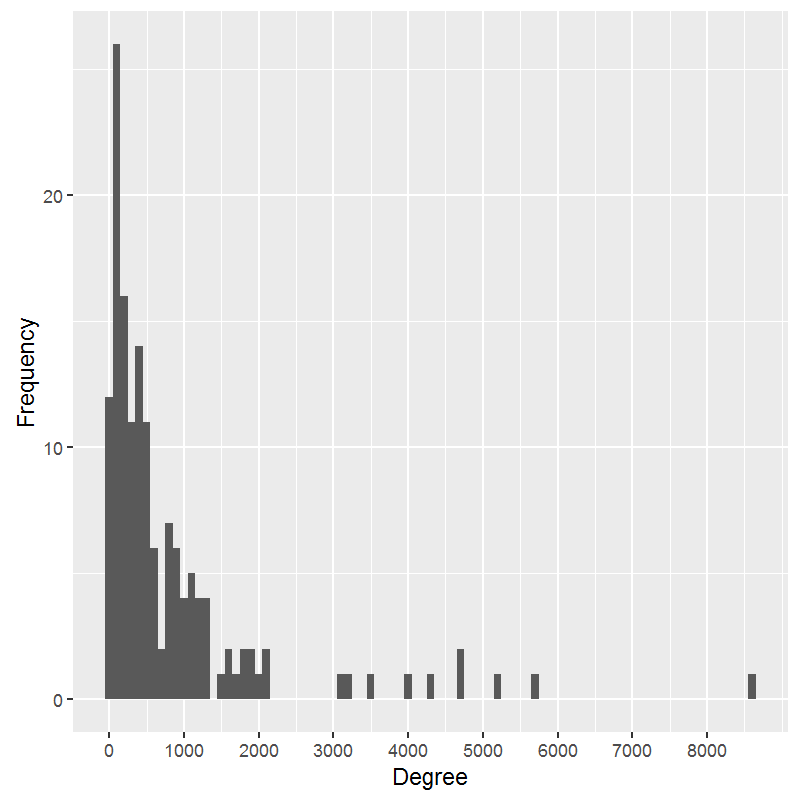
\includegraphics[height=8.33333in]{images/deg_freq.png}}{Degree Frequency}}\label{degree-frequency}

\newpage

\subsubsection{Figure B2 Degree Cumulative
Frequency}\label{figure-b2-degree-cumulative-frequency}

\section{\texorpdfstring{\protect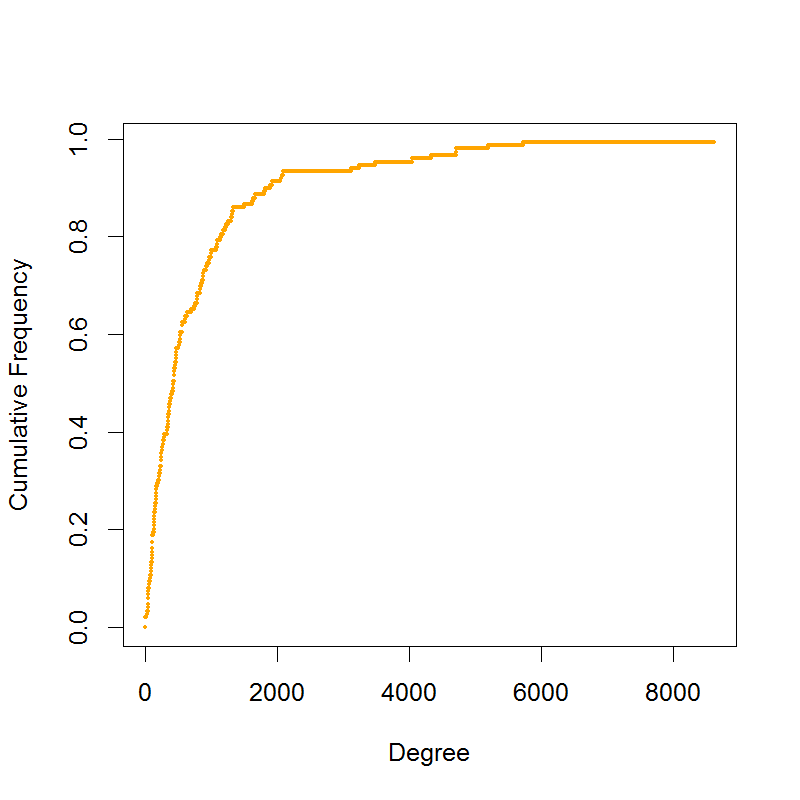
\includegraphics[height=8.33333in]{images/deg_cumfreq.png}}{Degree Cumulative Frequency}}\label{degree-cumulative-frequency}

\newpage

\subsubsection{Figure B3 Raw Network of Enron
Emails}\label{figure-b3-raw-network-of-enron-emails}

\section{\texorpdfstring{\protect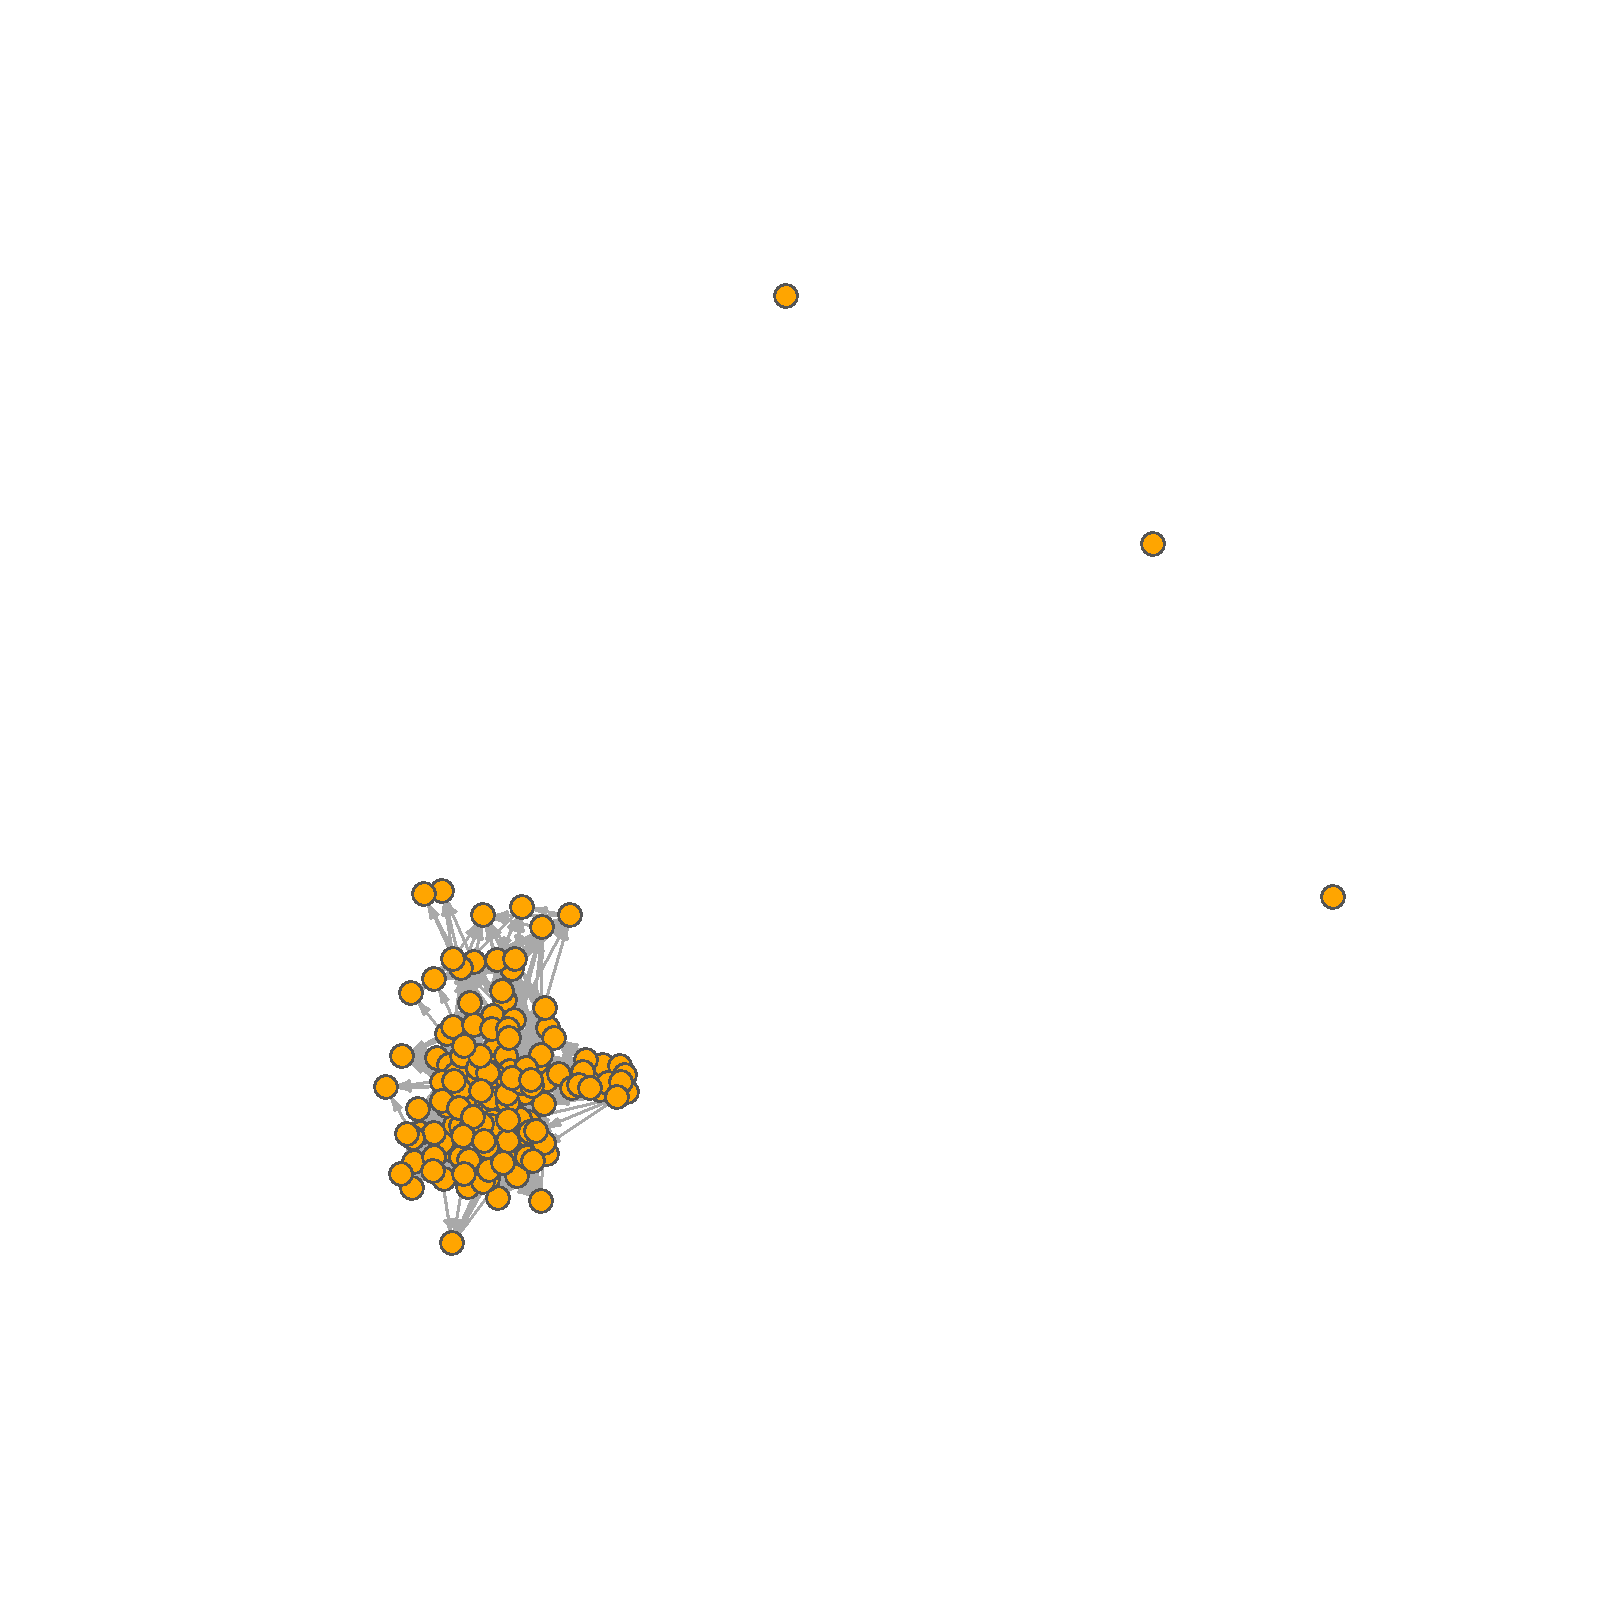
\includegraphics[height=12.50000in]{images/n_raw.png}}{Network of Enron Emails}}\label{network-of-enron-emails}

\newpage

\subsubsection{Figure B4 Network of Enron Emails (Emails sent
TO)}\label{figure-b4-network-of-enron-emails-emails-sent-to}

\section{\texorpdfstring{\protect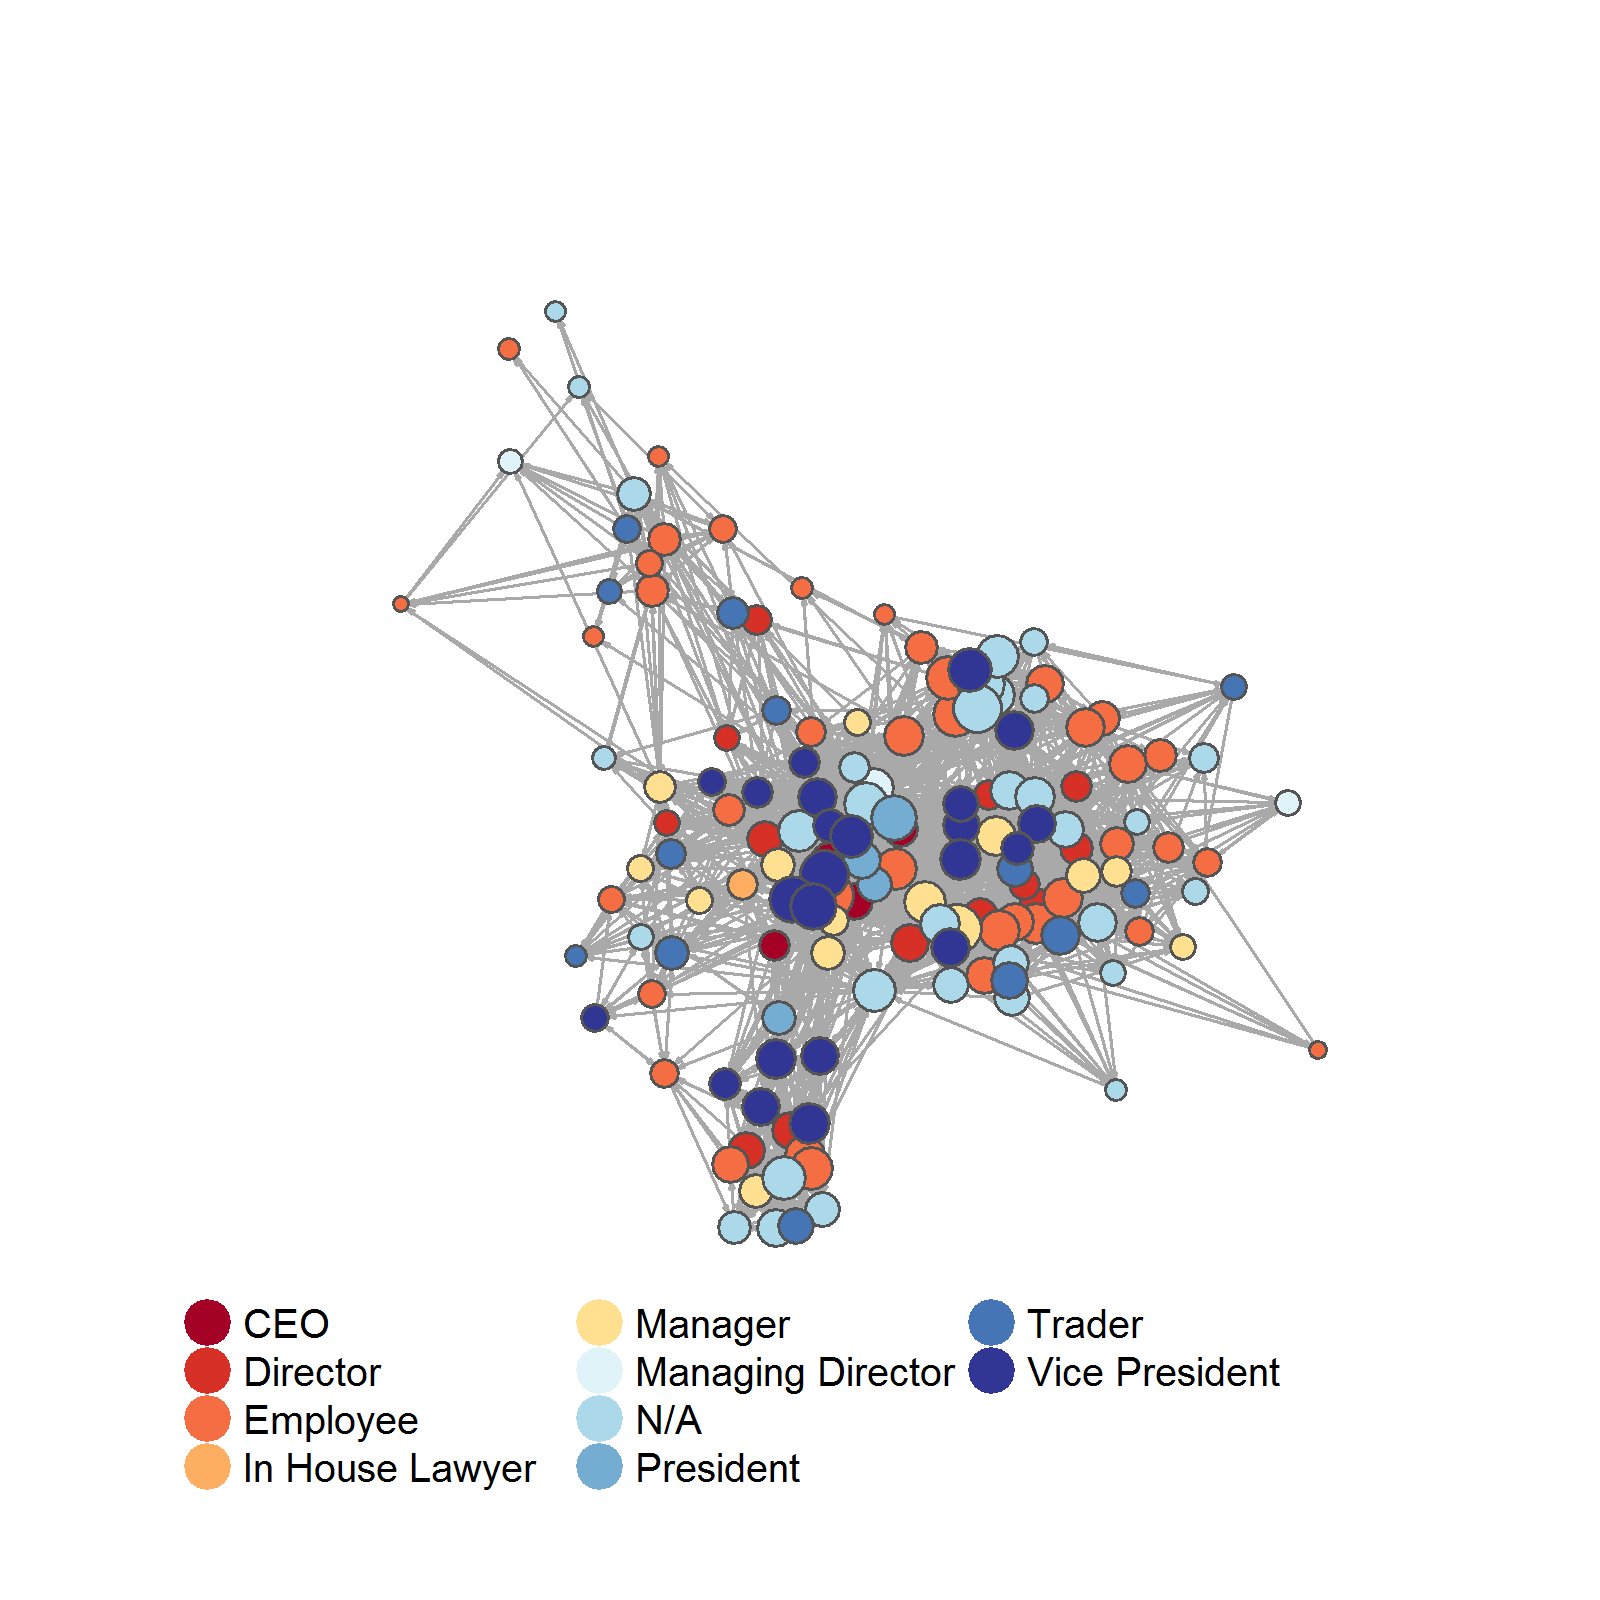
\includegraphics[height=12.50000in]{images/n_to.png}}{Network of Enron Emails}}\label{network-of-enron-emails-1}

\newpage

\subsubsection{Figure B5 Network of Enron Emails (Greater than 200
Emails sent
TO)}\label{figure-b5-network-of-enron-emails-greater-than-200-emails-sent-to}

\section{\texorpdfstring{\protect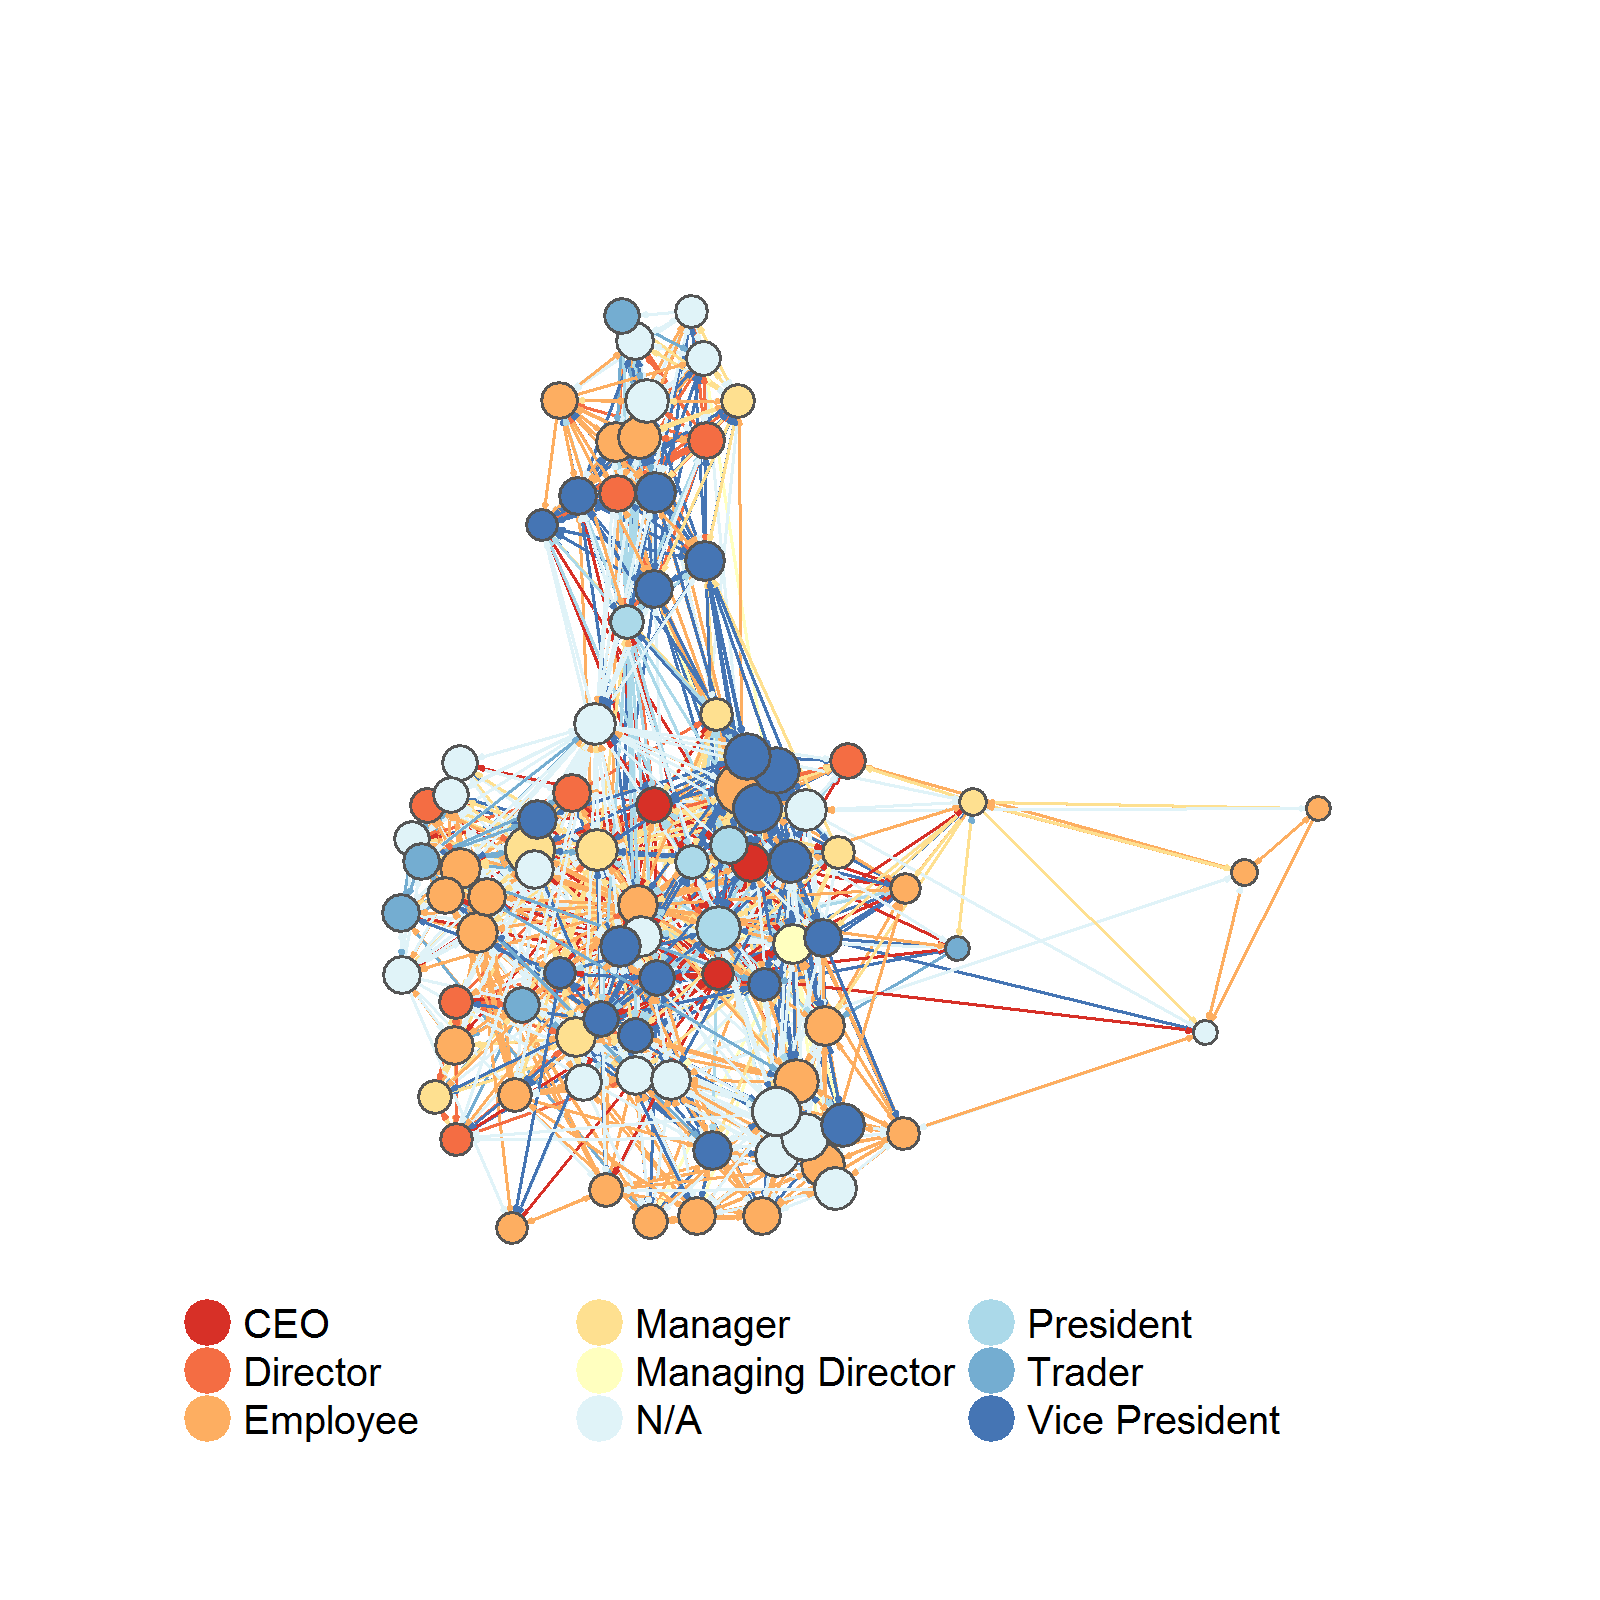
\includegraphics[height=12.50000in]{images/n_to_ge200.png}}{Network of Enron Emails}}\label{network-of-enron-emails-2}

\newpage

\subsubsection{Figure B6 Network of Enron Emails (Emails sent TO over
2000)}\label{figure-b6-network-of-enron-emails-emails-sent-to-over-2000}

\section{\texorpdfstring{\protect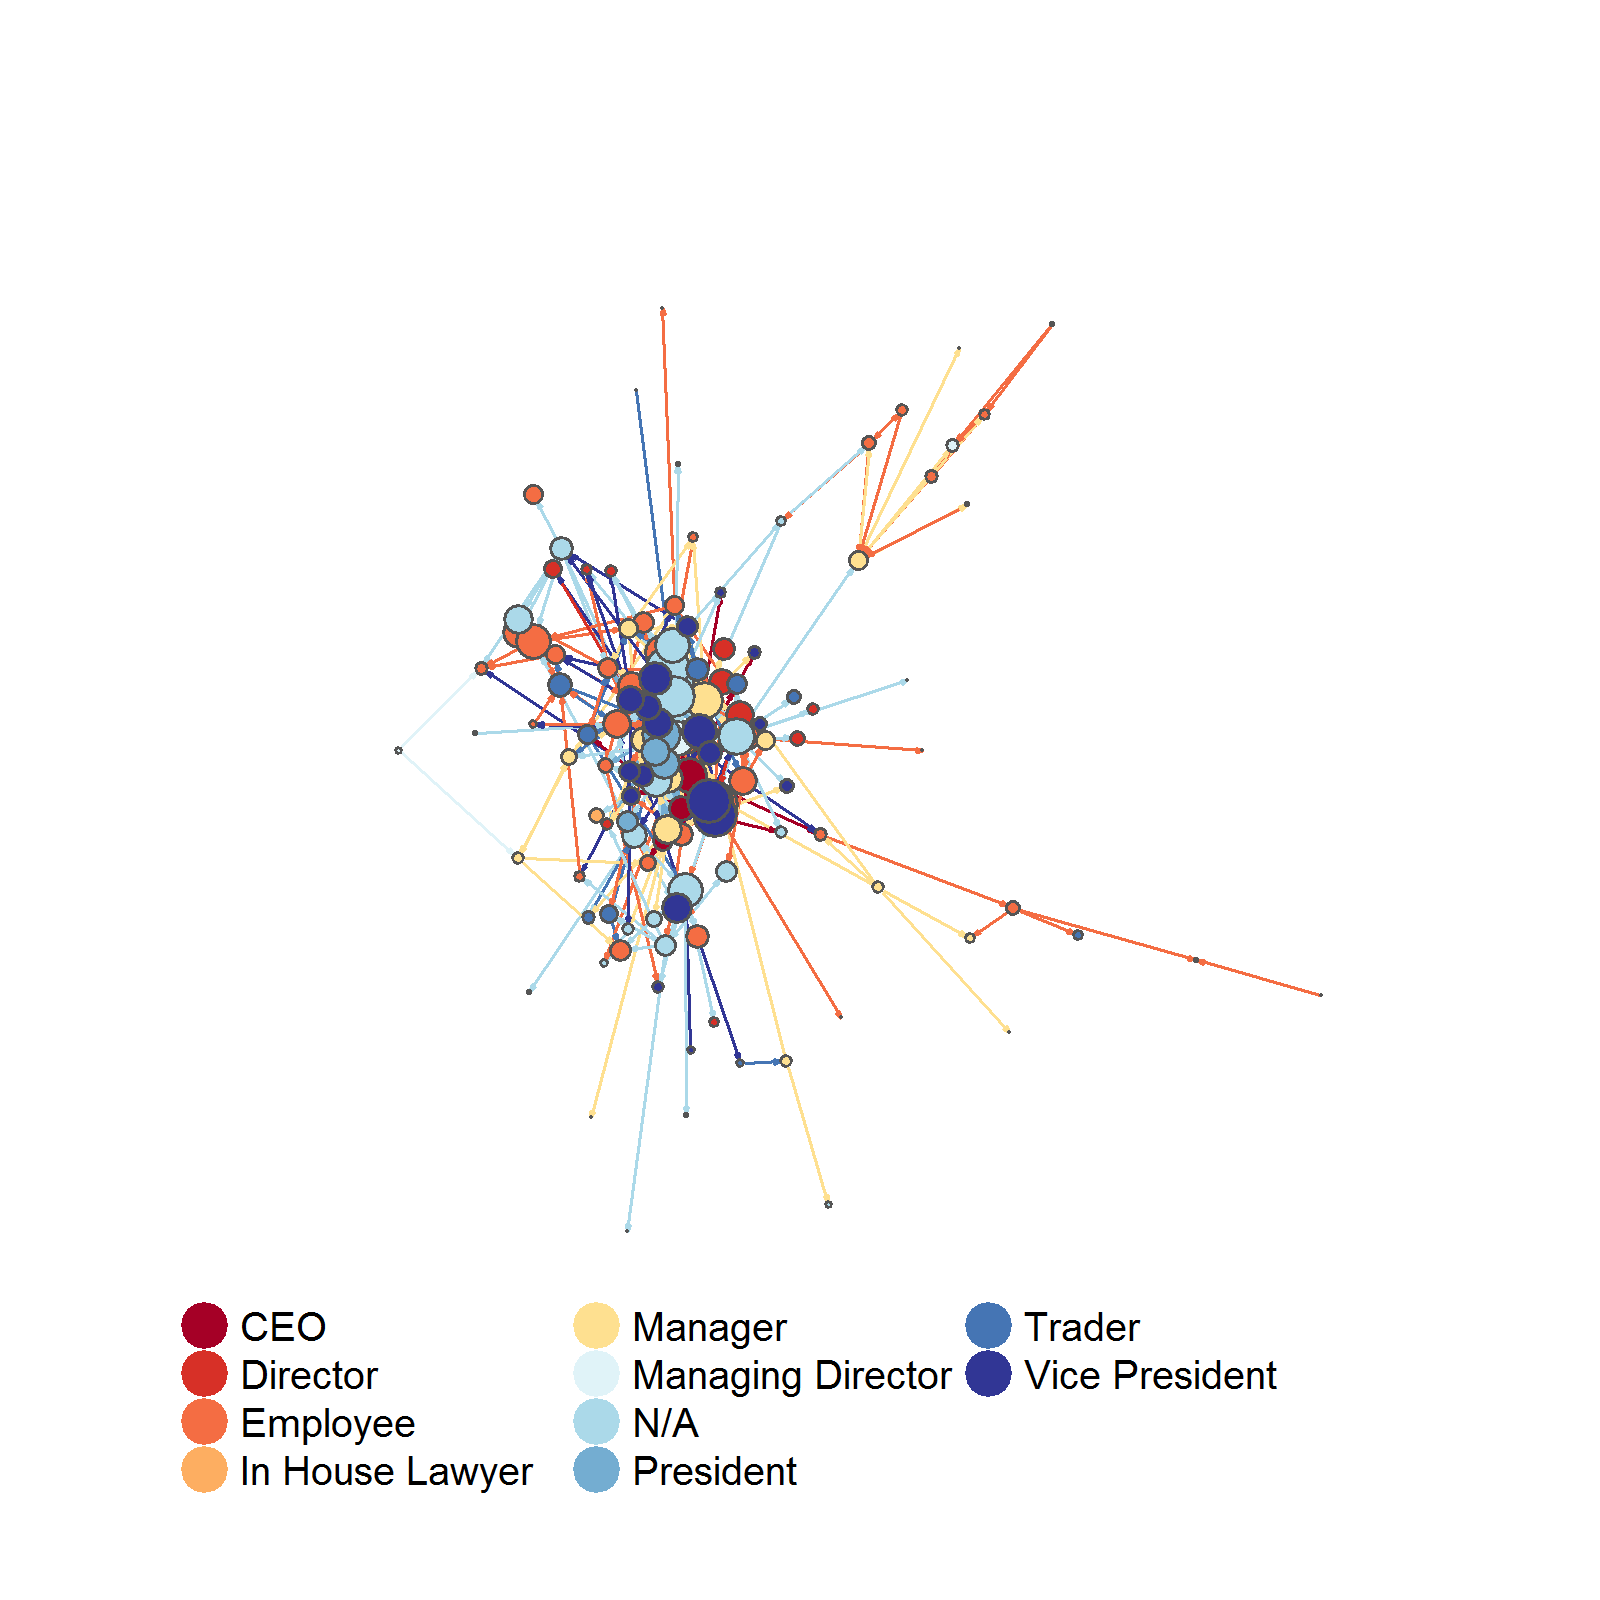
\includegraphics[height=12.50000in]{images/n_to_00.png}}{Network of Enron Emails}}\label{network-of-enron-emails-3}

\newpage

\subsubsection{Figure B7 Network of Enron Emails (Emails sent TO over
2000)}\label{figure-b7-network-of-enron-emails-emails-sent-to-over-2000}

\section{\texorpdfstring{\protect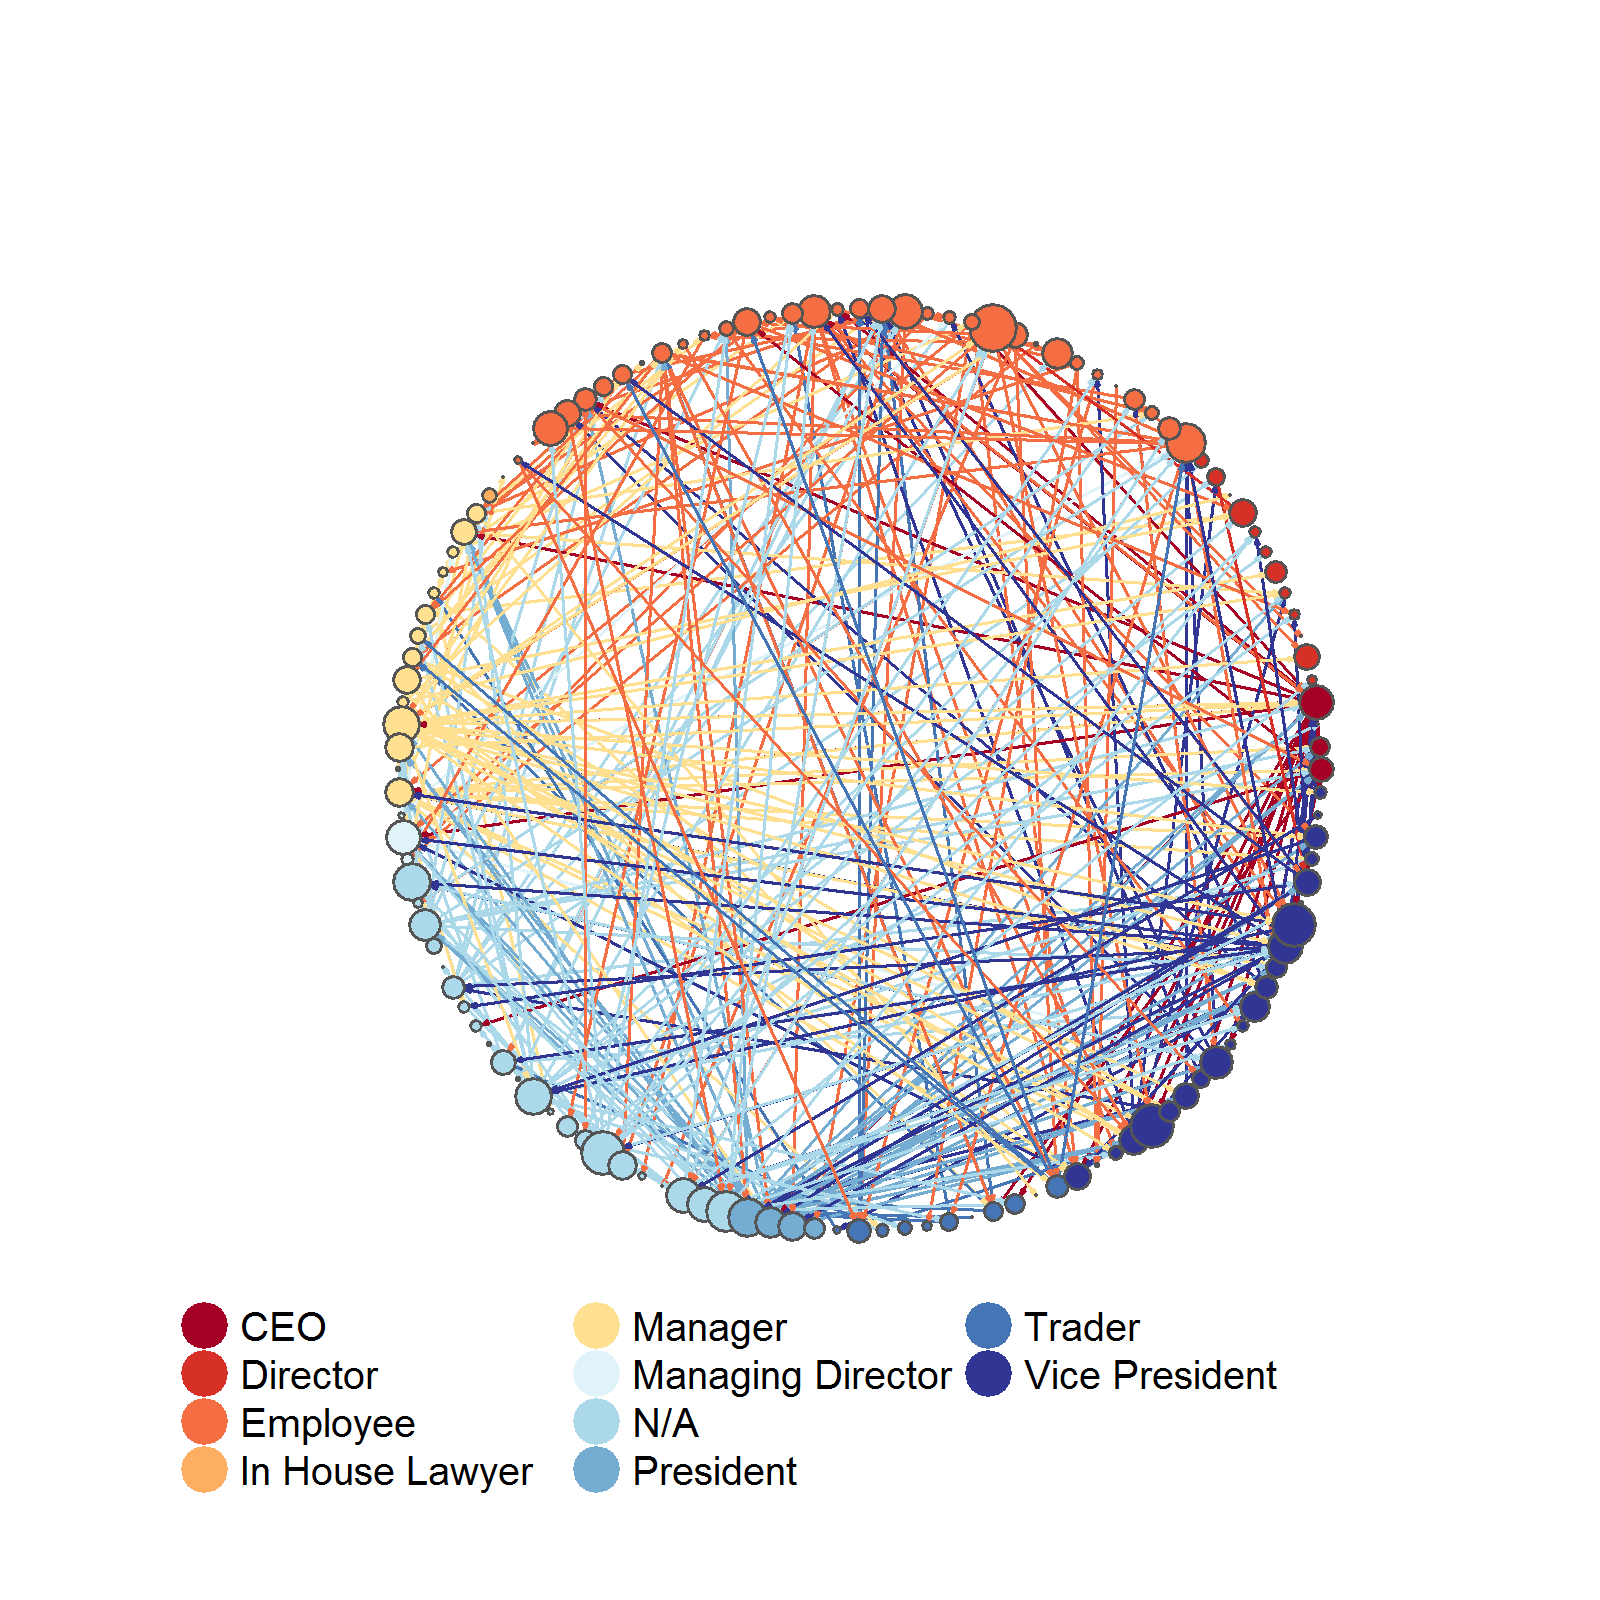
\includegraphics[height=12.50000in]{images/n_to_00e.png}}{Network of Enron Emails}}\label{network-of-enron-emails-4}

\newpage

\subsubsection{Figure B8 Network of Enron Emails (Emails sent TO over
2001)}\label{figure-b8-network-of-enron-emails-emails-sent-to-over-2001}

\section{\texorpdfstring{\protect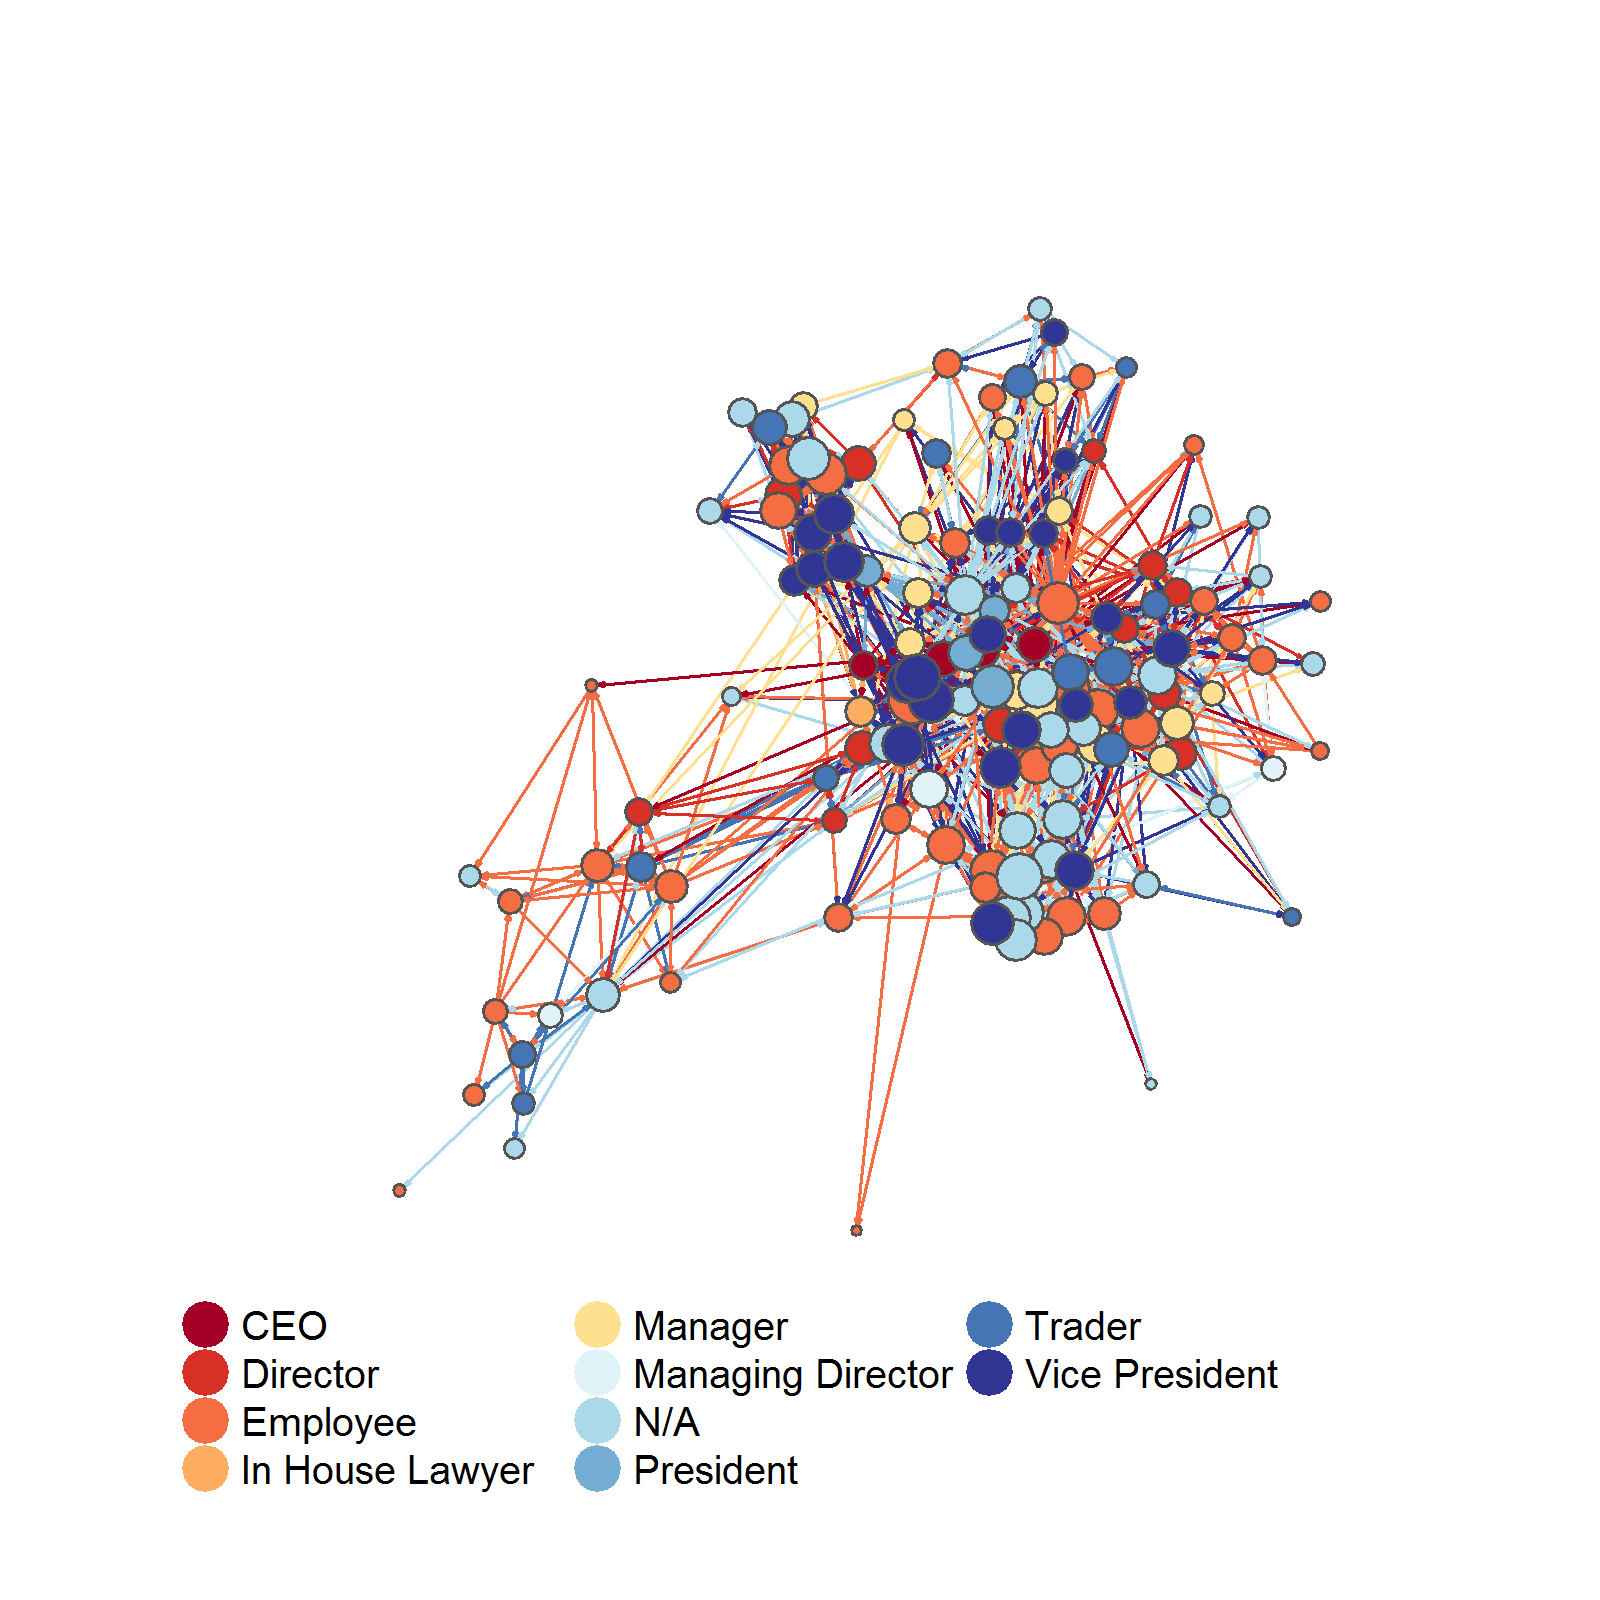
\includegraphics[height=12.50000in]{images/n_to_01.png}}{Network of Enron Emails}}\label{network-of-enron-emails-5}

\newpage

\subsubsection{Figure B9 Network of Enron Emails (Emails sent TO over
2001)}\label{figure-b9-network-of-enron-emails-emails-sent-to-over-2001}

\section{\texorpdfstring{\protect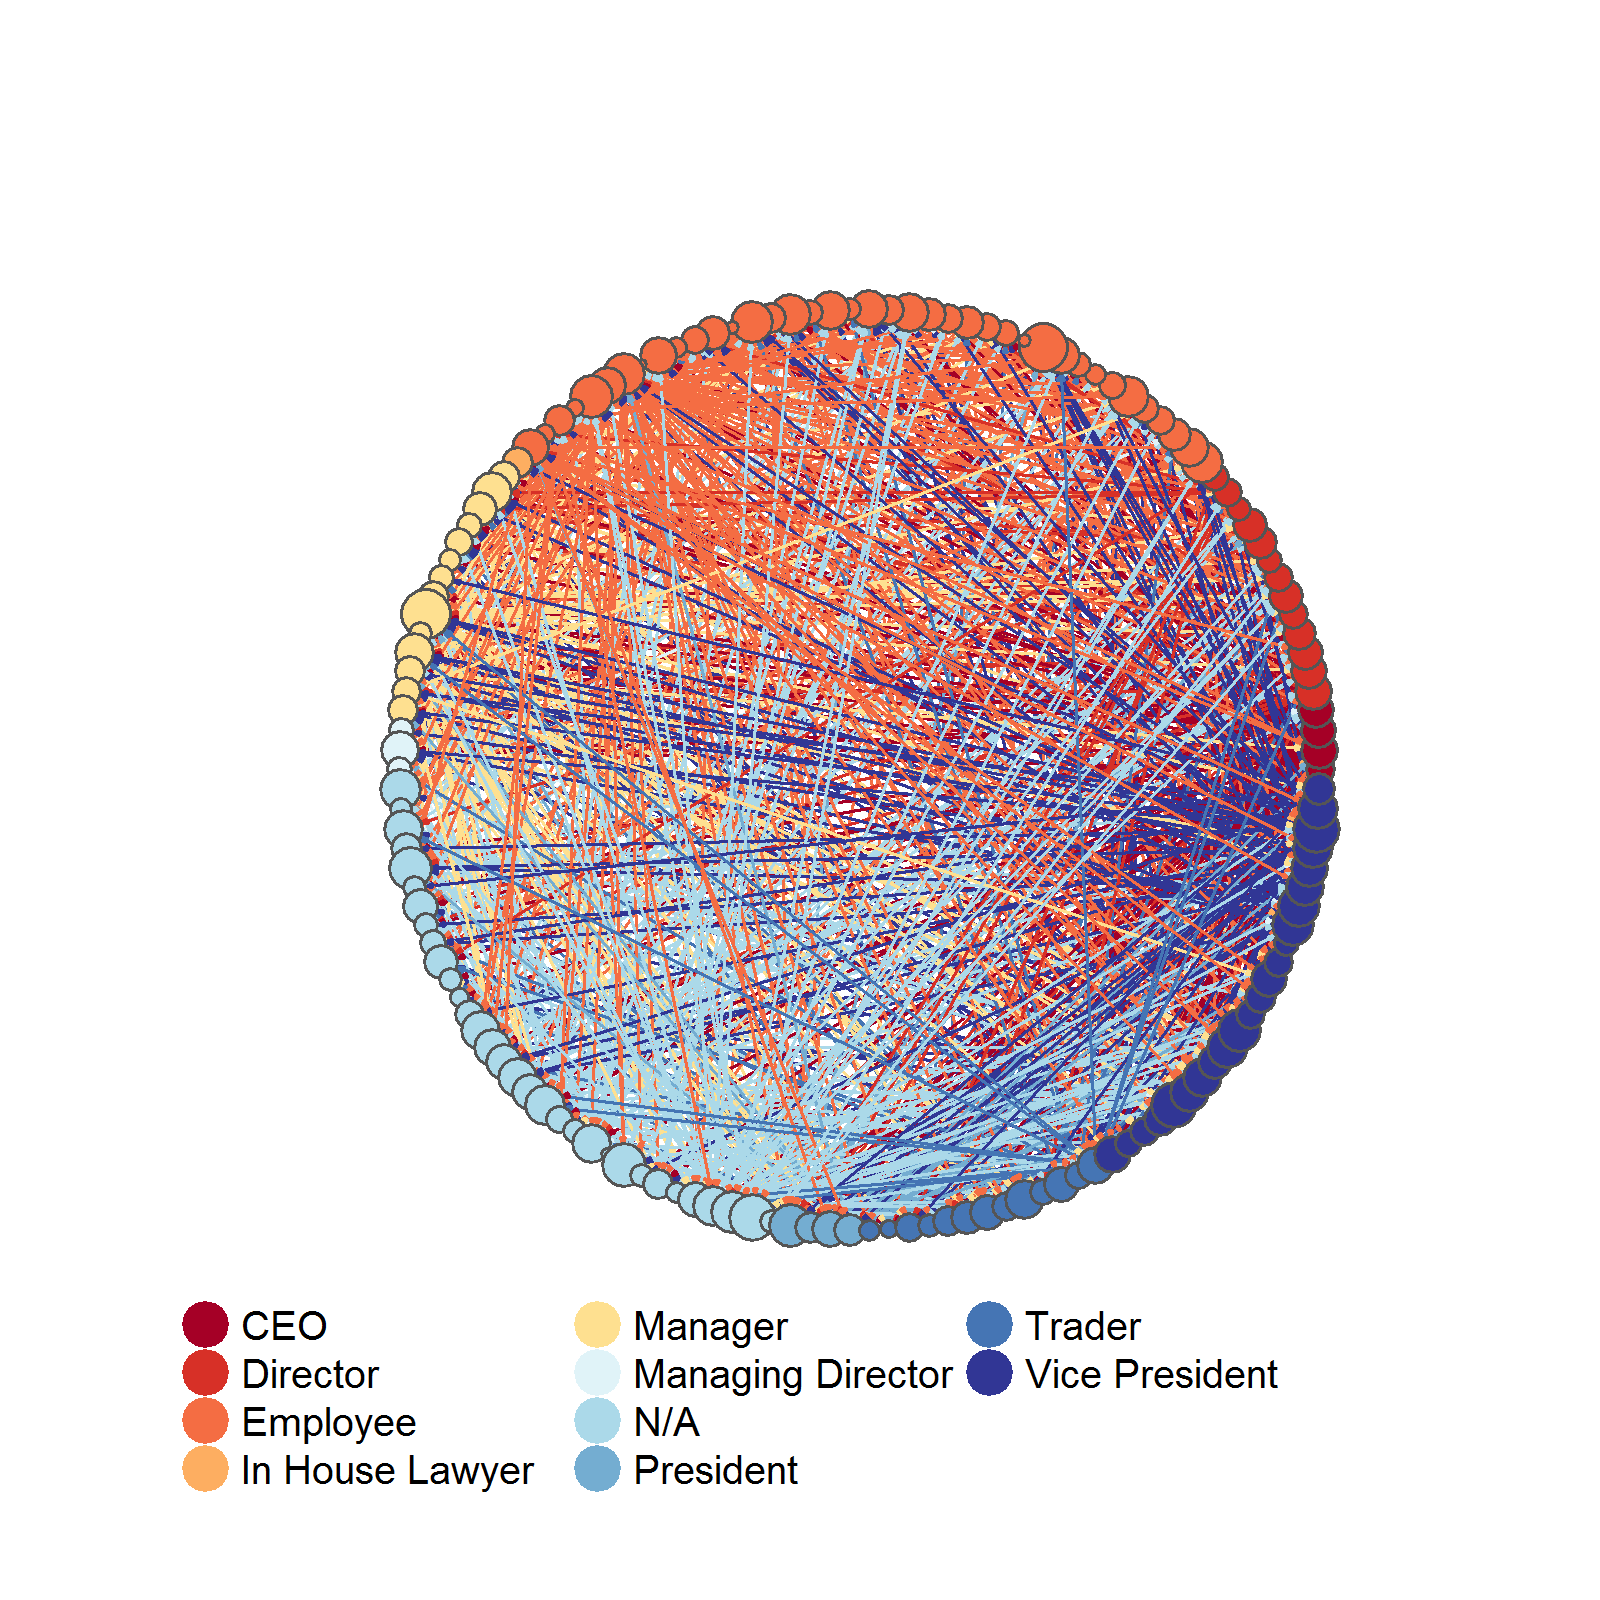
\includegraphics[height=12.50000in]{images/n_to_01e.png}}{Network of Enron Emails}}\label{network-of-enron-emails-6}

\newpage

\subsubsection{Figure B10 Network of Enron Emails (Emails sent TO over
2002)}\label{figure-b10-network-of-enron-emails-emails-sent-to-over-2002}

\section{\texorpdfstring{\protect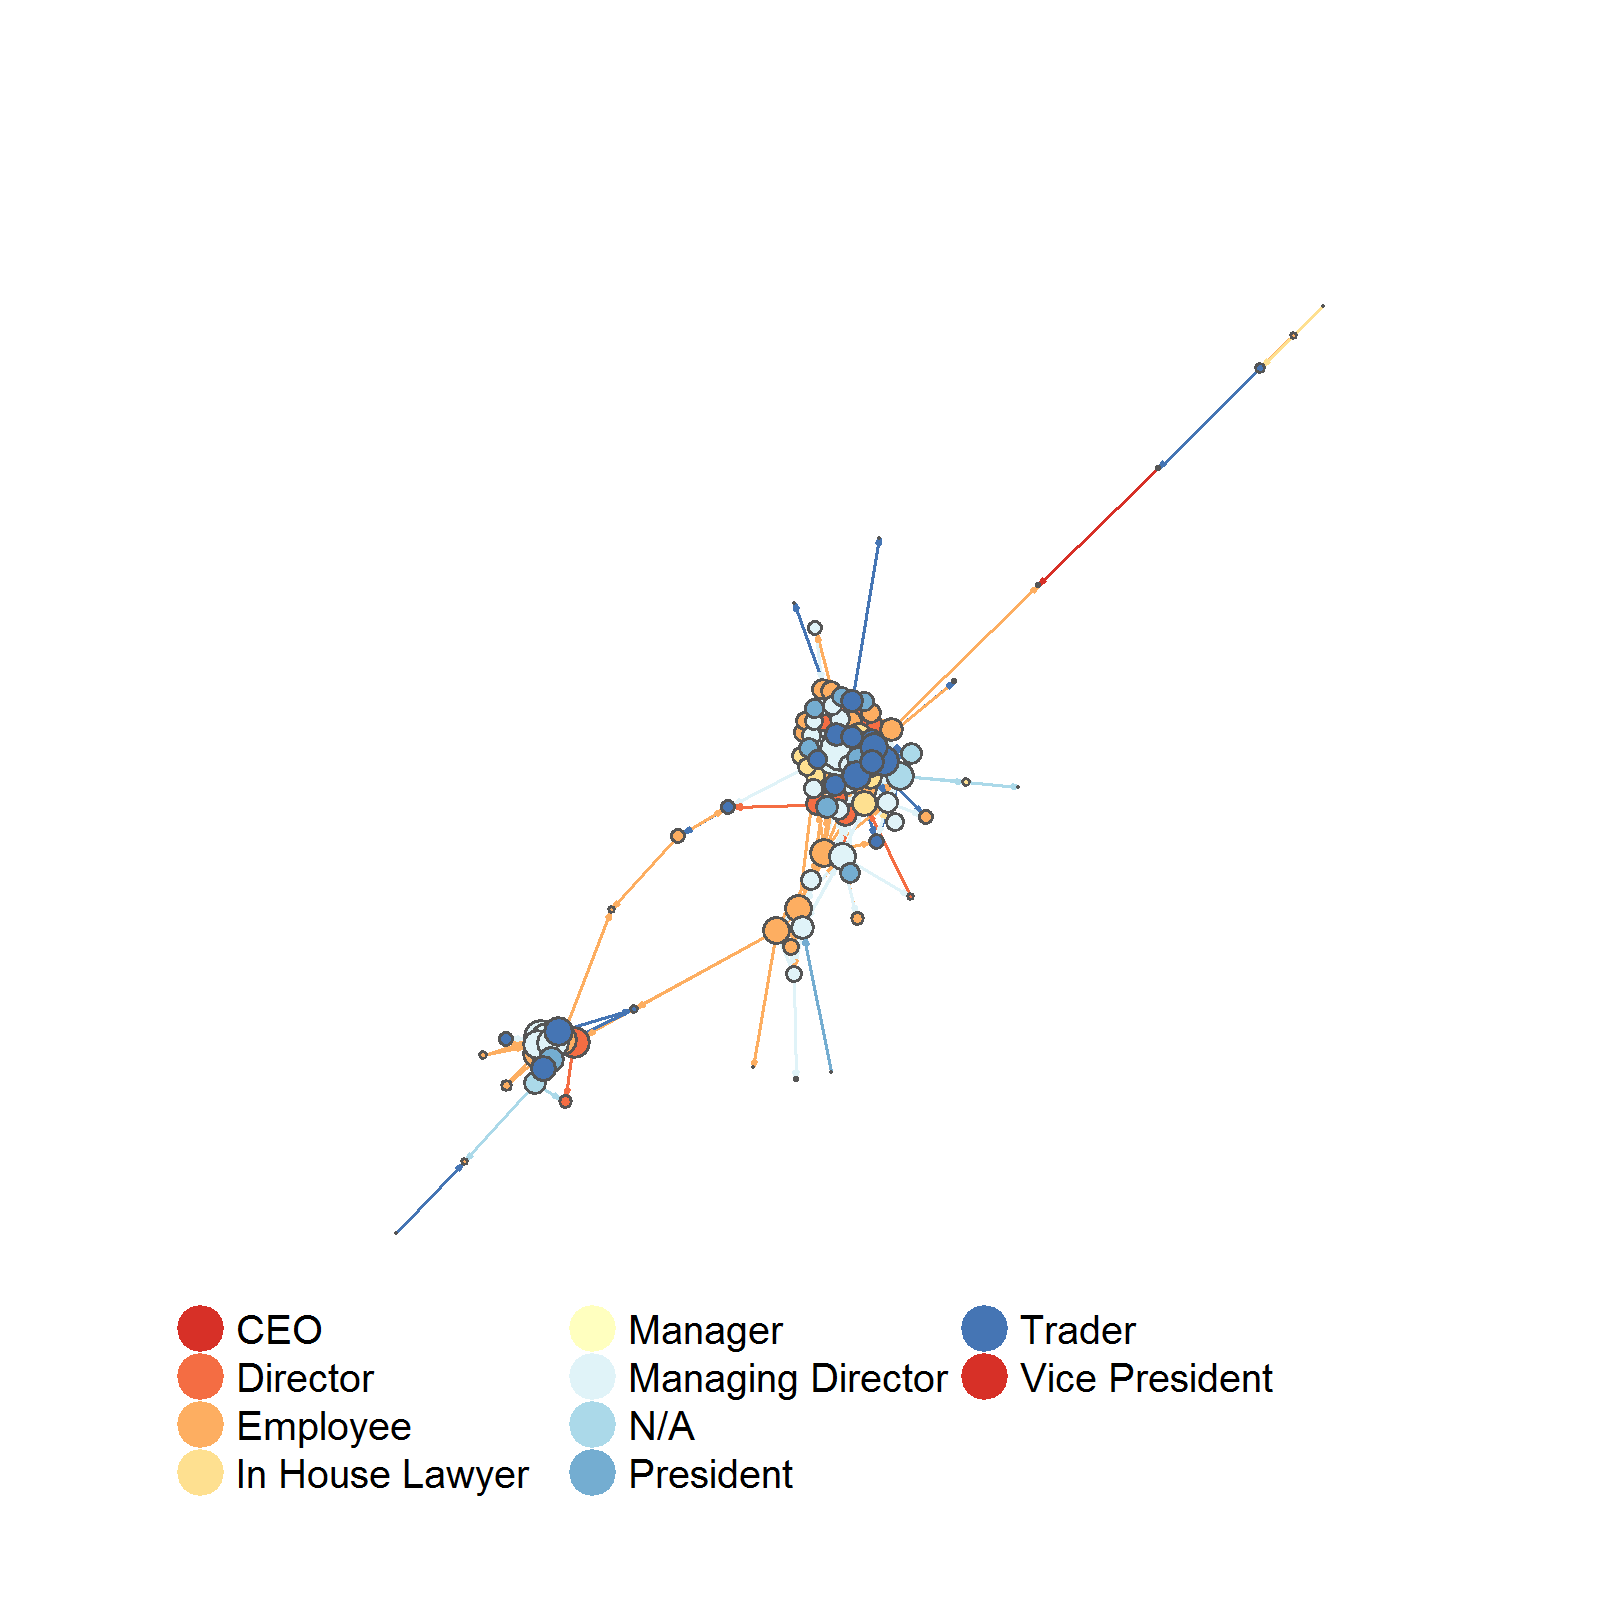
\includegraphics[height=12.50000in]{images/n_to_02.png}}{Network of Enron Emails}}\label{network-of-enron-emails-7}

\newpage

\subsubsection{Figure B11 Network of Enron Emails (Emails sent TO over
2002)}\label{figure-b11-network-of-enron-emails-emails-sent-to-over-2002}

\section{\texorpdfstring{\protect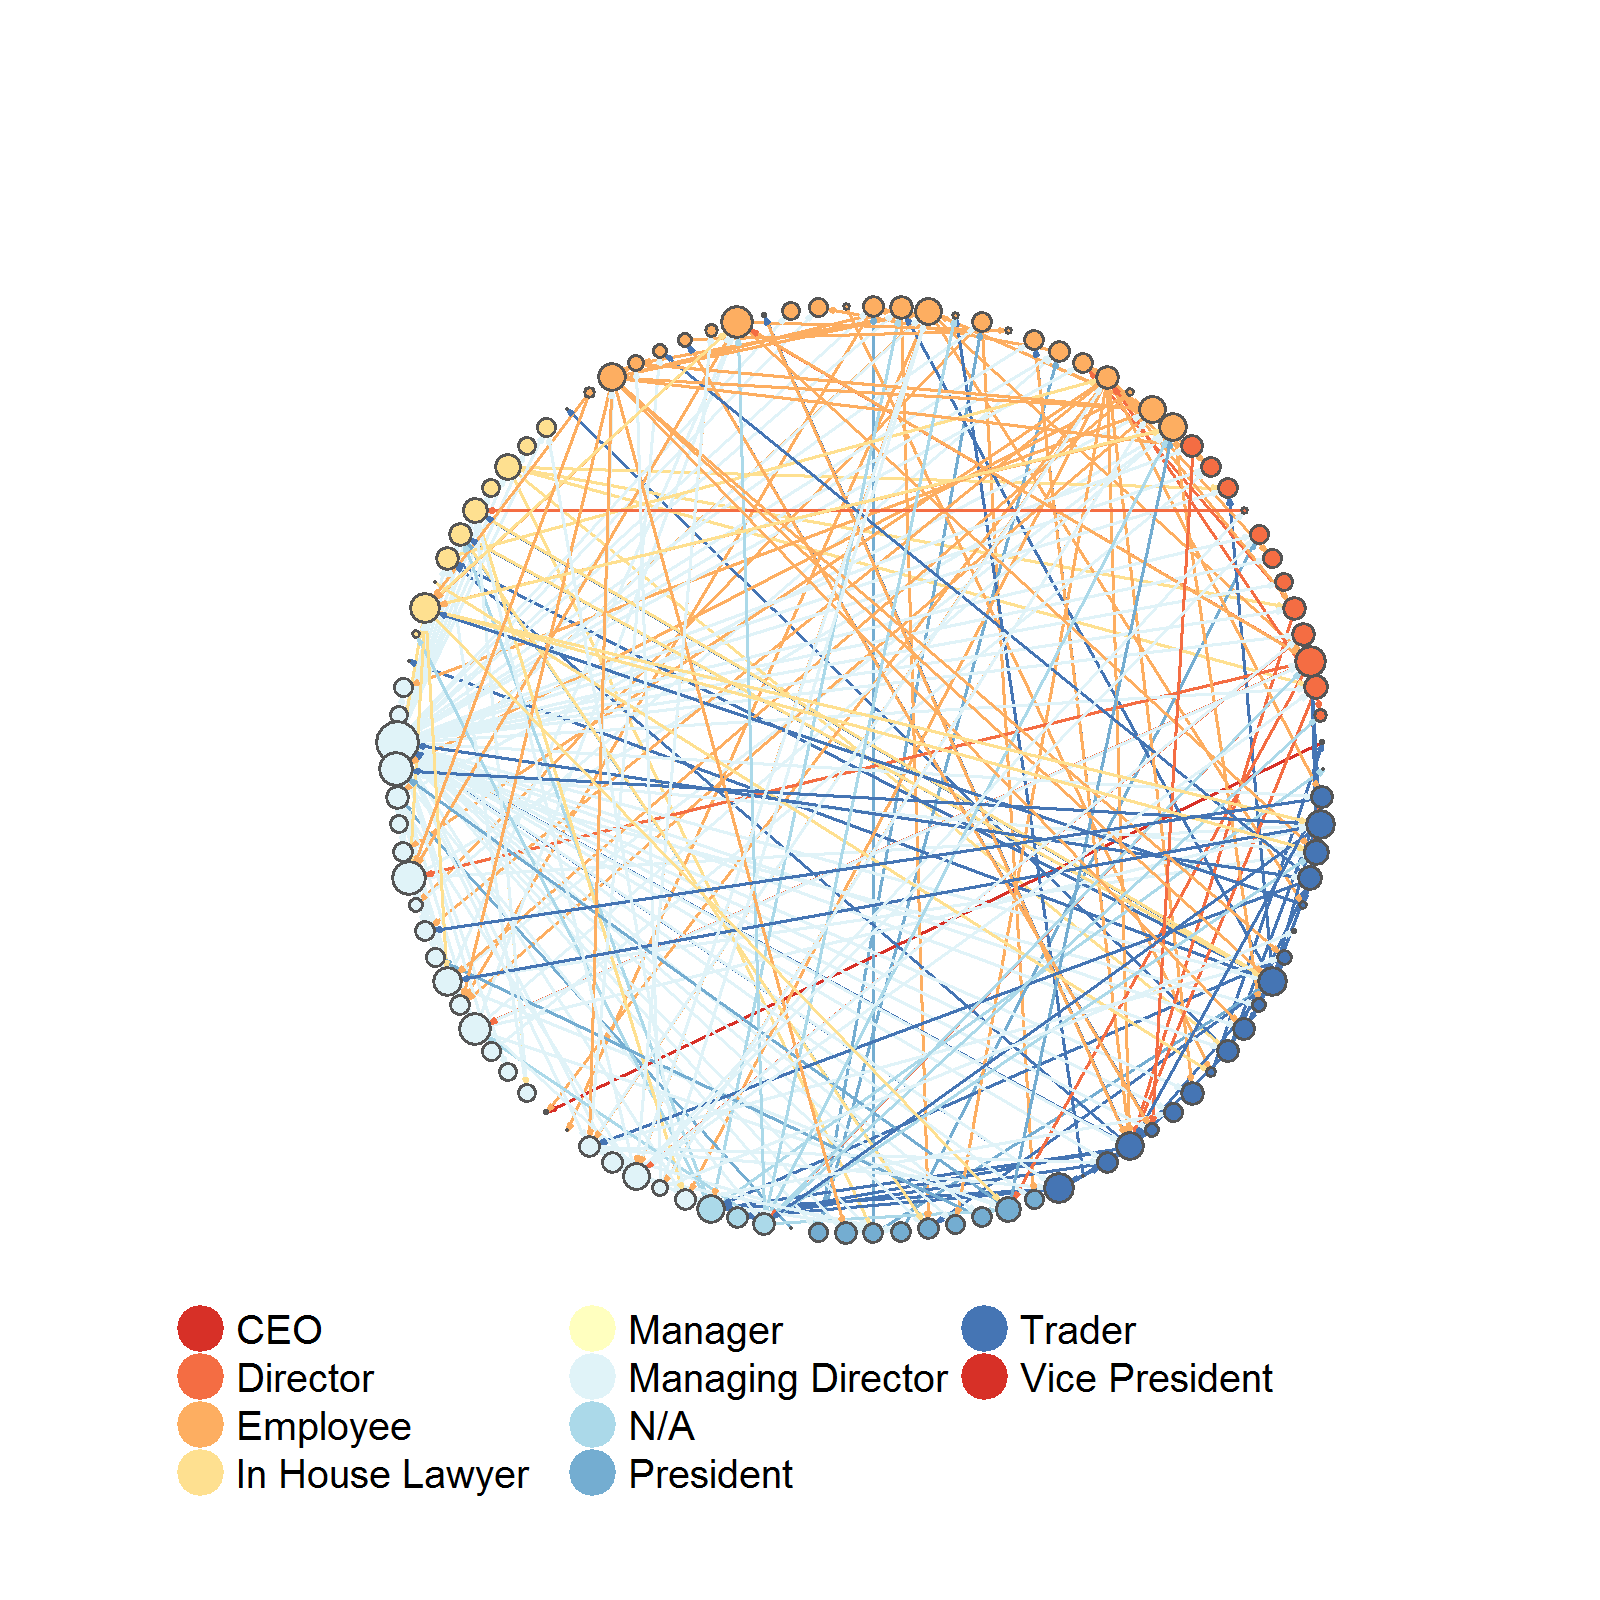
\includegraphics[height=12.50000in]{images/n_to_02e.png}}{Network of Enron Emails}}\label{network-of-enron-emails-8}

\newpage

\subsubsection{Figure B12 Network of Enron Emails (Nodes sized by Hub
Score)}\label{figure-b12-network-of-enron-emails-nodes-sized-by-hub-score}

\section{\texorpdfstring{\protect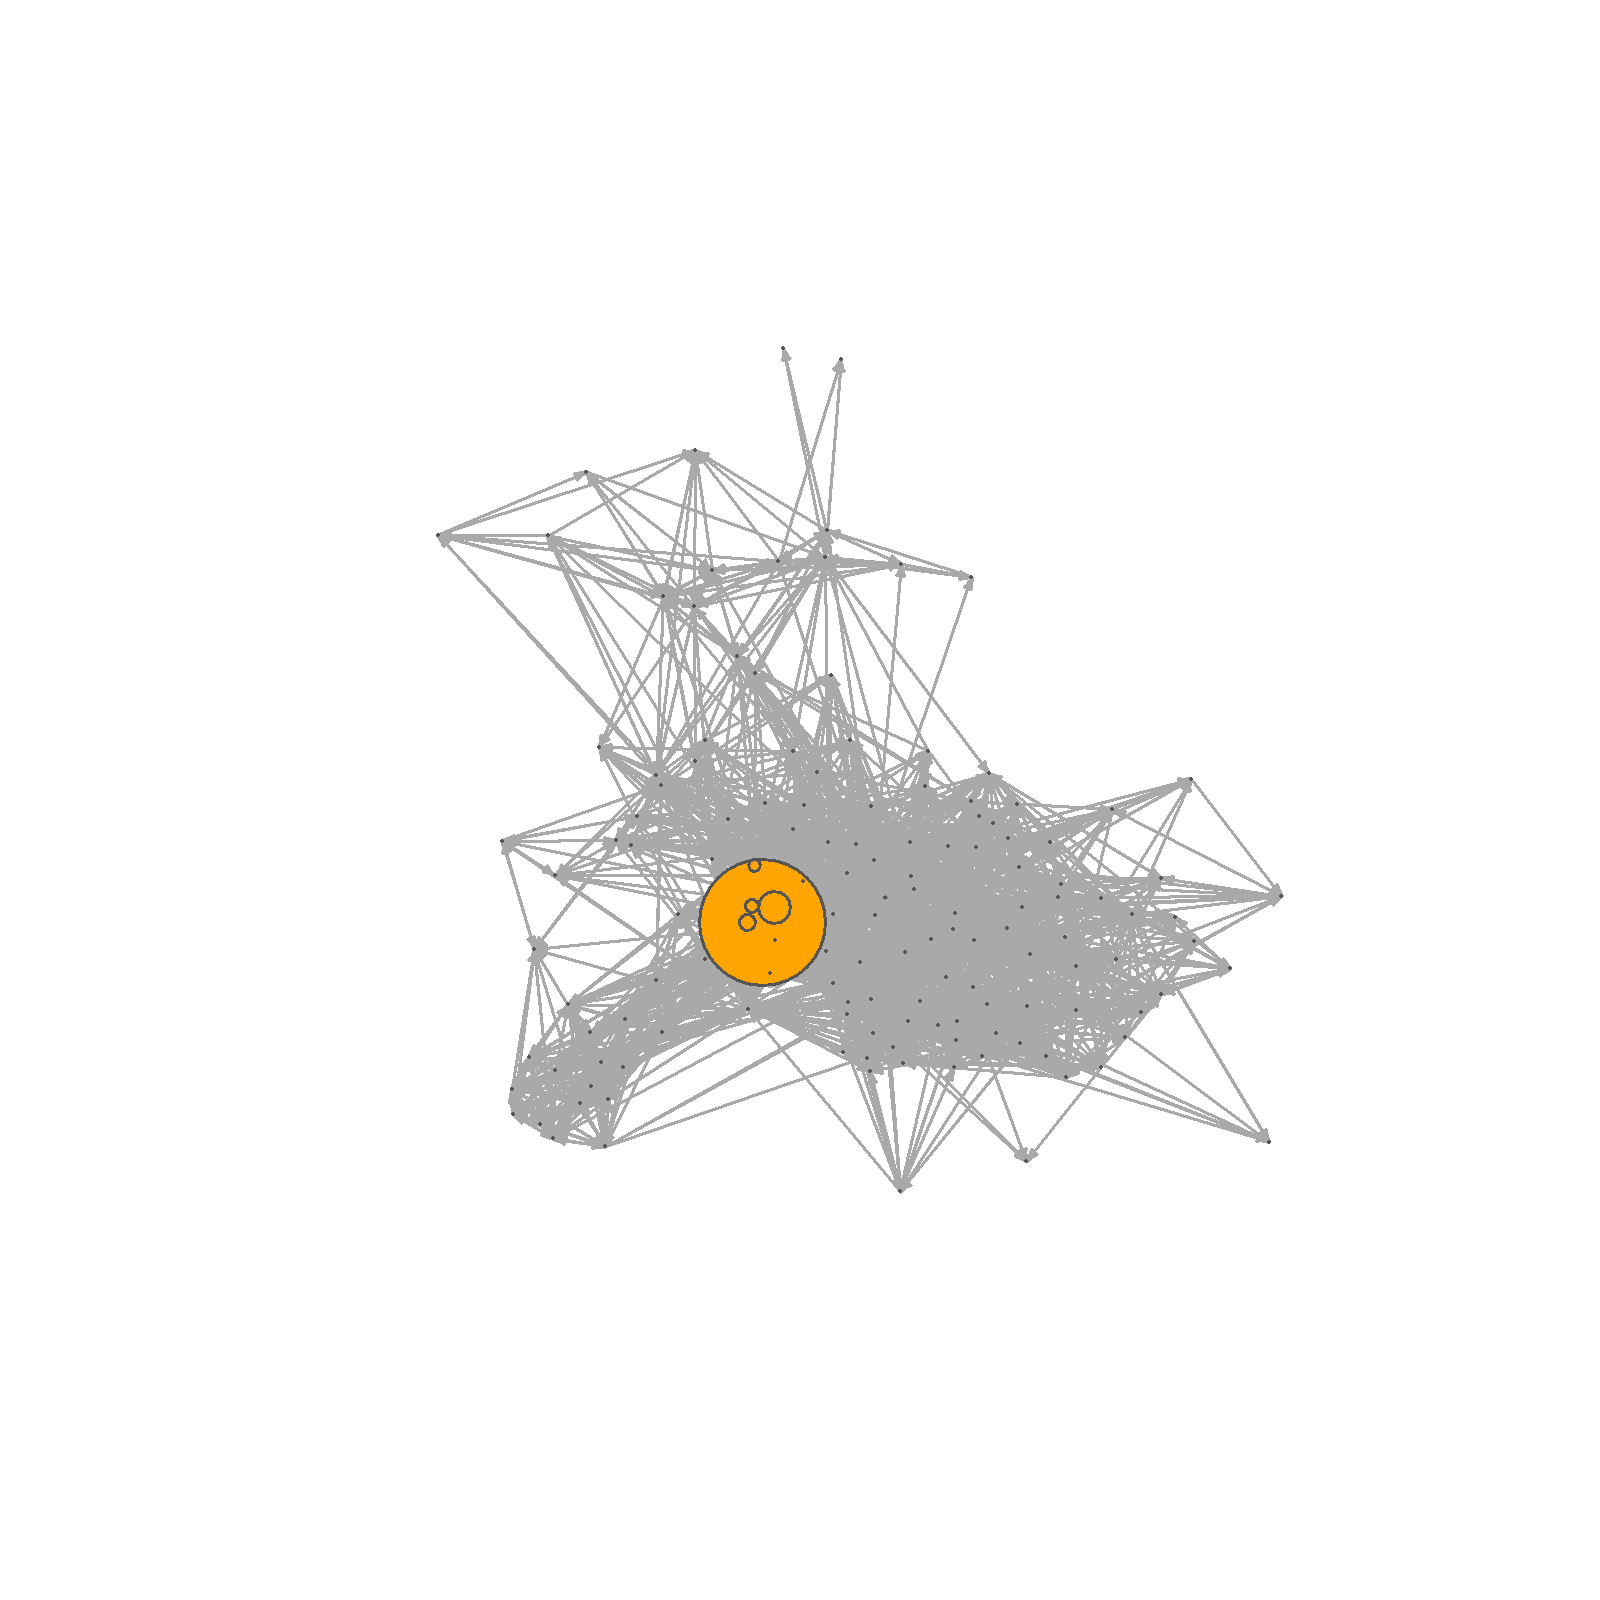
\includegraphics[height=12.50000in]{images/n_hs.png}}{Network of Enron Emails}}\label{network-of-enron-emails-9}

\newpage

\subsubsection{Figure B13 Network of Enron Emails (Nodes sized by
Authority
Score)}\label{figure-b13-network-of-enron-emails-nodes-sized-by-authority-score}

\section{\texorpdfstring{\protect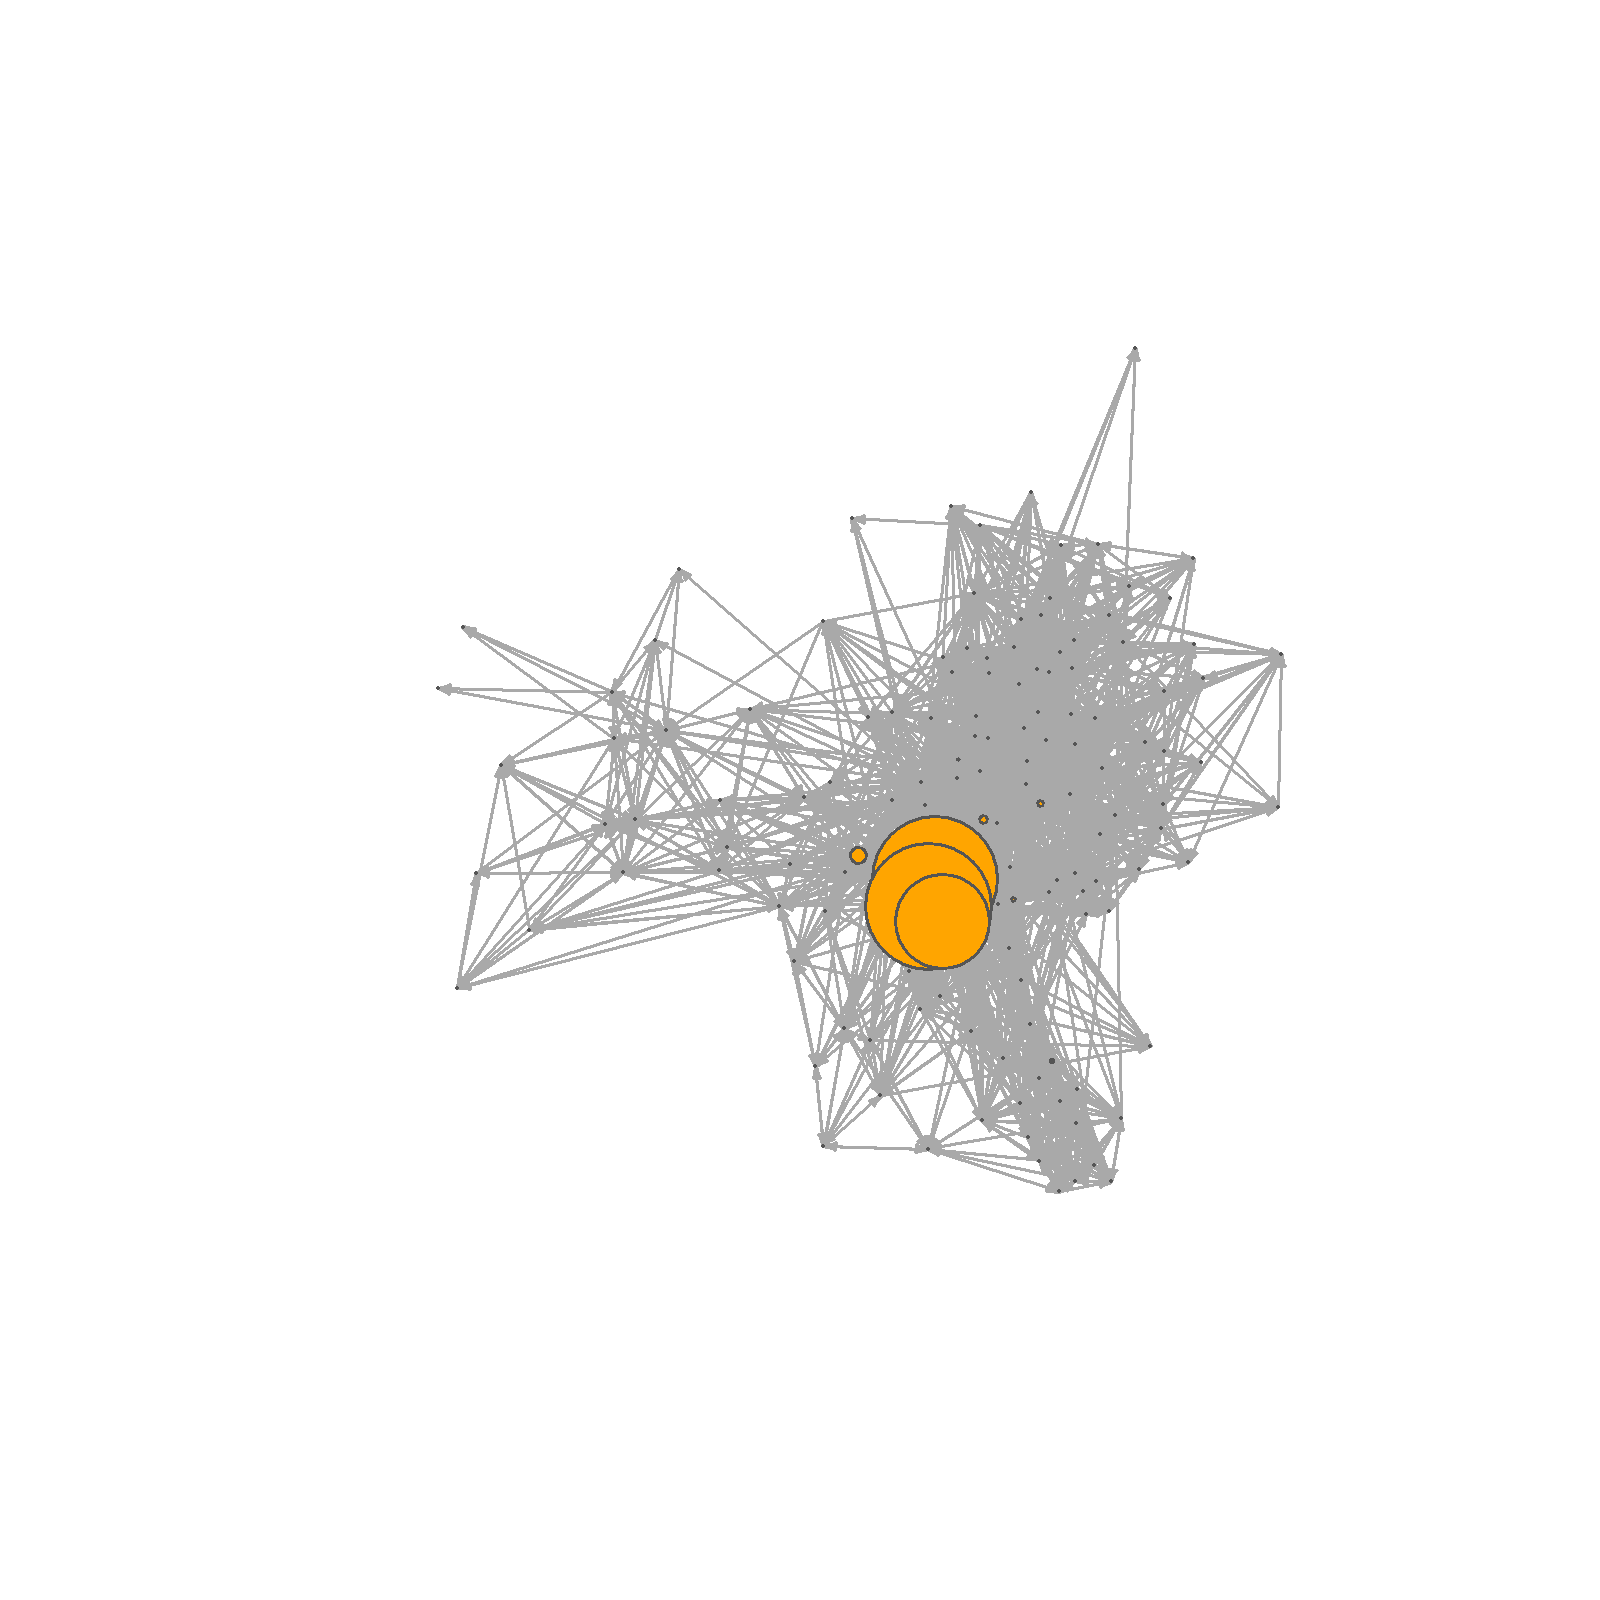
\includegraphics[height=12.50000in]{images/n_as.png}}{Network of Enron Emails}}\label{network-of-enron-emails-10}

\newpage

\section*{References}\label{references}
\addcontentsline{toc}{section}{References}

\hypertarget{refs}{}
\hypertarget{ref-Cohen2015}{}
Cohen, W. 2015. ``Enron Email Dataset.''
\url{http://www.cs.cmu.edu/~enron/}.

\hypertarget{ref-Klein1999}{}
Kleinberg, J. 1999. ``Hubs, Authorities, and Communities.''
\url{http://cs.brown.edu/memex/ACM_HypertextTestbed/papers/10.html}.

\hypertarget{ref-Schulz2015}{}
Schulz, A. 2015. ``Enron Data.''
\url{http://www.ahschulz.de/enron-email-data/}.


\end{document}
